\section{Design}

In this section, we would describe in detail the components of our system and the advantages of them.
The first component is a newly designed OS. 
It takes a micro-kernel structure but add network traffic into the kernel.
We also argue that this OS design can help us redesign the IoT network so that it's less vulnerable to attacks.

\subsection{\ritos}

As shown in \autoref{fig::design::os-overview}, our system take a micro-kernel architecture.
However, we intend to put the network stack inside the kernel.
Therefore, instead of providing \texttt{send()} and \texttt{recv()} system calls, we would make all POSIX APIs with regard to networks our system calls, including \texttt{socket()}, \texttt{recv()}, \texttt{send()}, etc.

In this \ritos, all processes are represented by an IP address with a port number. Inter-Process Communication(IPC) is no different than issuing a command over the internet.

\begin{figure}[h]
    \centering
    \resizebox{\linewidth}{!}{
        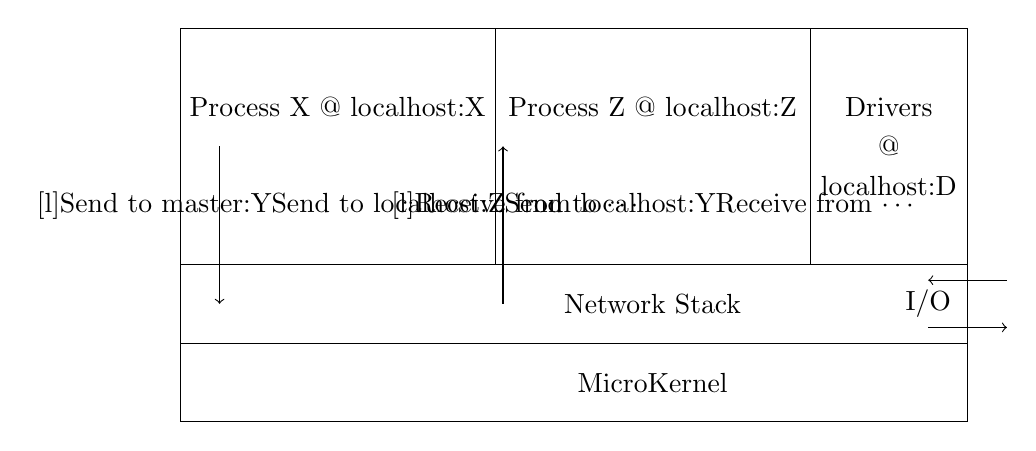
\begin{tikzpicture}
            \begin{scope}[local bounding box=IoTOS]
                \draw (0,0) rectangle (10, 5);
                \draw (0,1) rectangle (10, 2);
                \draw (0,2) rectangle (4, 5);
                \draw (4, 2) rectangle (8, 5);
                
                \node at (6, 0.5) {MicroKernel};
                \node at (6, 1.5) {Network Stack};
                
                \node at (2, 4) {Process X @ localhost:X};
                \node at (2, 2.75) {\makecell[l]{Send to master:Y \\ Send to localhost:Z  \\ Send to $\cdots$}};
                \draw[->] (0.5, 3.5) -- (0.5, 1.5);

                \node at (6, 2.75) {\makecell[l]{Receive from localhost:Y  \\ Receive from $\cdots$}};
                \draw[->] (4.1, 1.5) -- (4.1, 3.5);

                \node at (6, 4) { Process Z @ localhost:Z };
                \node at (9, 4) { Drivers };
                \node at (9, 3.5) { @ };
                \node at (9, 3) { localhost:D };
            \end{scope}
            
            IoTOS
            
            \node at (9.5, 1.5) {I/O};
            \draw[->] (9.5, 1.2) -- (10.5, 1.2);
            \draw[->] (10.5, 1.8) -- (9.5, 1.8);
        \end{tikzpicture}
    }
\caption{OS overview}
\label{fig::design::os-overview}
\end{figure}

\subsection{Redesign IoT Network}

As shown in \autoref{fig::design::system-overview}, different devices are connected to a master device which controls everything.
Instead of talking to different devices the user can only talk to the master device.
This design guarantees that even if a malicious hacker has all passphrases of a user, he can't do any harm until he controls the master device.
Since any slave device only talks to the master device, they can't temper with each other too.

\begin{figure*}[h]
    \centering
    \resizebox{\linewidth}{!}{
        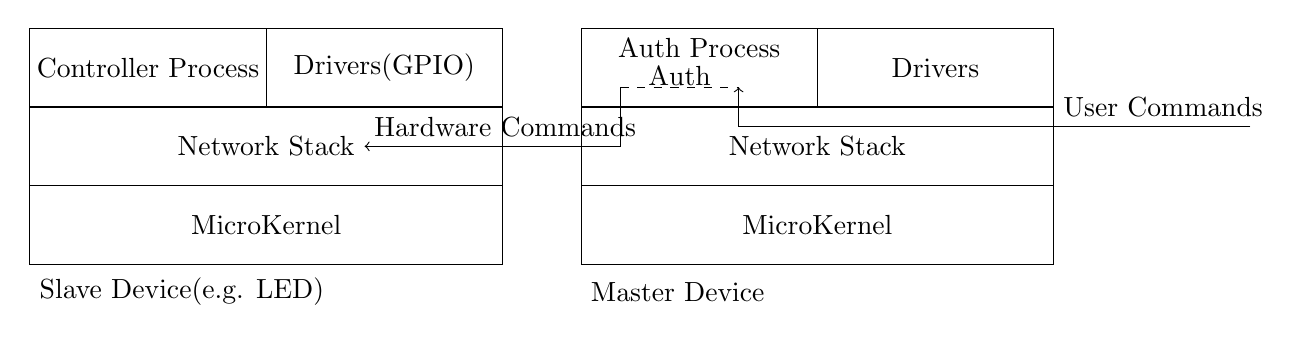
\begin{tikzpicture}
            \begin{scope}[local bounding box=IoTOS]
                \node[anchor=west] at (0, -.35) {Slave Device(e.g. LED)};

                \draw (0,0) rectangle (6, 3);
                \draw (0,1) rectangle (6, 2);
                \draw (0,2) rectangle (3, 3);
                \draw (3,3) rectangle (6, 3);
                
                \node at (3, 0.5) {MicroKernel};
                \node at (3, 1.5) {Network Stack};
                
                \node at (1.5, 2.5) {Controller Process};

                \node at (4.5, 2.5) {Drivers(GPIO)};
            \end{scope}
        
            \begin{scope}[shift = {(7, 0)}]
                \node[anchor=west] at (0, -.35) {Master Device};

                \draw (0,0) rectangle (6, 3);
                \draw (0,1) rectangle (6, 2);
                \draw (0,2) rectangle (3, 3);
                \draw (3,3) rectangle (6, 3);
                
                \node at (3, 0.5) {MicroKernel};
                \node at (3, 1.5) {Network Stack};
                
                \node at (1.5, 2.75) {Auth Process};

                \node at (4.5, 2.5) {Drivers};
            \end{scope}

            \draw[->] (7.5, 2.25) -- (7.5, 1.5) -- (4.25, 1.5);
            \node[anchor = west] at (4.25, 1.75) { Hardware Commands };
            %\node[anchor = west] at (4.25, 1.25) { HTTPS Encrypted };

            \draw[->] (15.5, 1.75) -- (9, 1.75) -- (9, 2.25);
            \node[anchor = west] at (13, 2) { User Commands };

            \draw[dashed] (7.5, 2.25) -- (9, 2.25);
            \node at (8.25, 2.4) { Auth };
        \end{tikzpicture}
    }
\caption{System overview}
\label{fig::design::system-overview}
\end{figure*}

\subsection{Authtication}

For a user to talk to the master device, an extra authentication needs to be done to guarantee that the "user" is not a hacker.
This process can be done using 2FA, i.e. One-time password(OTP), email confirmation, etc.